\documentclass[11pt]{article}

\usepackage[margin=1in]{geometry}
\usepackage[T1]{fontenc}
\usepackage[utf8]{inputenc}
\usepackage{lmodern}
\usepackage{microtype}
\usepackage{amsmath,amssymb}
\usepackage{booktabs}
\usepackage{array}
\newcolumntype{L}[1]{>{\raggedright\arraybackslash}p{#1}}
\usepackage{multirow}
\usepackage{float}
\usepackage{graphicx}
\usepackage{xcolor}
\usepackage{tikz}
\usetikzlibrary{positioning,arrows.meta,fit}
\usepackage[numbers,sort&compress]{natbib}
\usepackage[colorlinks=true,linkcolor=blue!50!black,citecolor=blue!50!black,urlcolor=blue!50!black]{hyperref}
\usepackage[capitalise,noabbrev]{cleveref}
\usepackage{enumitem}
\setlist{nosep,leftmargin=*}

\graphicspath{{figures/}}
\newcommand{\OS}{\textsc{os}}
\newcommand{\SR}{\textsc{sr}}
\newcommand{\vbar}{\bar{v}}
\newcommand{\na}{--}

\title{Four Ways to Navigate:\\An Empirical Study of Vision-and-Language Navigation Policies on a Single GPU}
\author{Shubh Jain\\[2pt]\small\url{https://github.com/ShubhJain007/vln-four-ways}}
\date{September 2026}

\begin{document}
\maketitle

\begin{abstract}
We study four ways of turning a pretrained vision-language or video model into an instruction-following navigation
policy for Vision-and-Language Navigation in continuous environments (R2R-CE). Every model is trained with low-rank
adapters on one 16\,GB consumer GPU:
(i)~a from-scratch reimplementation of LatentPilot, whose \emph{Pilot Token} is trained to predict the visual embedding
two steps ahead and is fed back as a recurrent latent;
(ii)~a waypoint-\emph{pointing} policy whose image-space prediction drives a bearing controller;
(iii)~the pretrained action stream of the Cosmos3-Edge video world model, used zero-shot as a diffusion policy; and
(iv)~the reasoning tower of the same model, fine-tuned to output the next command from eight seconds of egocentric video.

At this scale the LatentPilot objective fails the method's own gate. The learned Pilot Token predicts future frames
$2.25\times$ better than an identity control, yet reaches the goal less often (oracle success 10.7\% vs.\ 17.3\%,
$n{=}150$). We trace this to a loss balance that drifts by an order of magnitude during training.

Pointing supervision benefits from label corrections, more data, frame history, and reading the STOP decision from
intermediate layers. With these it reaches a strict self-stop success rate of \textbf{31.3\%} (SPL 25.4) on 150 unseen
episodes, the best true success rate in the study. The zero-shot diffusion policy recovers ego-motion from video (yaw
correlation 0.84--0.99) but follows full instructions only weakly (oracle success 7.5\%). The fine-tuned reasoner reaches
the goal region most often (oracle success \textbf{47.5\%} on 40 episodes), but it almost never stops there.

Across all four approaches, stopping rather than reaching is the bottleneck. Offline probes ranked candidate models
incorrectly twice, and silent implementation errors changed results as much as any modelling choice. Code, logs,
figures and rollout videos are released.
\end{abstract}

%=====================================================================================================================
\section{Introduction}
%=====================================================================================================================

Vision-and-Language Navigation (VLN) asks an embodied agent to follow a natural-language route instruction through an
unseen building using only egocentric observations~\citep{anderson2018r2r}. The continuous-environment variant R2R-CE
removes the navigation graph. The agent issues low-level actions (move forward 0.25\,m, turn 15\textdegree, stop) in
the Habitat simulator~\citep{krantz2020vlnce,savva2019habitat} on Matterport3D scans~\citep{chang2017mp3d}.

Recent systems build VLN policies on large pretrained video-language models~\citep{zhang2024navid,zhang2024uninavid,
cheng2024navila}, and recent work proposes giving such policies an internal model of the future.
LatentPilot~\citep{latentpilot} trains a \emph{Pilot Token} to predict the next-but-one visual embedding and carries it
across steps, so that the policy ``dreams ahead''. It reports 51.7--54.0\% success on R2R-CE with a 7B model. Its code
was not released.

This report asks a practical question: \emph{on a single 16\,GB GPU, which way of turning a pretrained model into a
VLN policy actually works, and why do the others fail?} We compare four architectures that differ in \emph{what the
model is asked to output} (\cref{fig:arch}):
\begin{enumerate}
  \item \textbf{LatentPilot}: discrete action tokens plus a recurrent latent trained to predict future frames;
  \item \textbf{pointing}: an image-space waypoint and a STOP probability, converted to actions by a geometric
        controller, following Robostral Navigate~\citep{robostral};
  \item \textbf{Cosmos3-Edge action model}: ego-pose trajectories sampled from a pretrained video diffusion
        model~\citep{nvidia2026cosmos3edge,nvidia2025cosmoswfm};
  \item \textbf{Cosmos3-Edge reasoner}: a natural-language command from a fine-tuned video reasoner.
\end{enumerate}

Our contributions are:
\begin{itemize}
  \item A from-scratch reimplementation of LatentPilot, and a controlled test of its central claim. With a learned
        future predictor versus an identity control and everything else fixed, it fails at 2B parameters and 1,665
        episodes. We diagnose the failure as loss-balance drift (\cref{sec:res-lp}).
  \item A pointing policy that reaches 31.3\% strict success, with ablations over data scale, history and layer
        fusion. A layer-wise probe shows that the STOP decision is decodable mid-network (AUC 0.72) but not at the
        output layer (0.44) (\cref{sec:res-pt}).
  \item The first, to our knowledge, closed-loop evaluation of Cosmos3-Edge's action stream and reasoner as VLN policies,
        including a guidance analysis and the finding that offline next-action accuracy does not predict closed-loop
        success (\cref{sec:res-edge,sec:res-rs}).
  \item A catalogue of silent implementation errors, each measured, that change results without raising an error
        (\cref{sec:gotchas}), and a strict evaluation protocol that separates reaching the goal from stopping at it
        (\cref{sec:protocol}).
\end{itemize}

\begin{figure}[t]
\centering
\tikzset{
  box/.style={draw, rounded corners=2pt, align=center, font=\scriptsize, inner sep=3pt, minimum height=5mm},
  inbox/.style={box, fill=gray!10},
  mdlbox/.style={box, fill=blue!10},
  outbox/.style={box, fill=orange!15},
  arr/.style={-{Latex[length=1.6mm]}, thick},
  lbl/.style={font=\scriptsize\bfseries, anchor=west}
}
\begin{minipage}{0.49\linewidth}\centering
\resizebox{\linewidth}{!}{\begin{tikzpicture}[node distance=3mm and 4mm]
  \node[inbox] (f) {frame $o_t$};
  \node[inbox, below=of f] (x) {instruction $x$};
  \node[inbox, below=of x] (z) {Pilot slot $z_{t-1}$};
  \node[mdlbox, right=6mm of x, minimum height=18mm, text width=17mm] (b) {Cosmos-Reason2-2B\\LoRA, explicit mRoPE};
  \node[outbox, right=6mm of b.north east, anchor=north west] (a) {FWD / L / R / STOP};
  \node[outbox, right=6mm of b.south east, anchor=south west] (g) {$z_t = G_\psi(h^{pil}_t)$};
  \draw[arr] (f) -- (b.west |- f); \draw[arr] (x) -- (b); \draw[arr] (z) -- (b.west |- z);
  \draw[arr] (b.east |- a) -- (a); \draw[arr] (b.east |- g) -- (g);
  \draw[arr, dashed] (g.south) -- ++(0,-3.5mm) -| (z.south);
  \node[font=\scriptsize, below=5mm of b] {$\mathcal{L}_{pil} = \|z_t - \vbar_{t+2}\|^2$};
\end{tikzpicture}}\par
{\small (a) LatentPilot: latent dream-ahead token}
\end{minipage}\hfill
\begin{minipage}{0.49\linewidth}\centering
\begin{tikzpicture}[node distance=3mm and 4mm]
  \node[inbox, text width=17mm] (f) {$o_t$ + 2 history frames};
  \node[inbox, below=of f, text width=17mm] (x) {instruction $x$};
  \node[mdlbox, right=5mm of f.south east, anchor=west, minimum height=12mm, text width=16mm, yshift=-1.5mm] (b)
       {Cosmos-Reason2-2B\\LoRA};
  \node[mdlbox, right=4mm of b, text width=13mm] (h) {head on layers 23/26/28};
  \node[outbox, below=4mm of h, text width=17mm] (c) {bearing controller: turn if $|\theta|>7.5^\circ$};
  \node[outbox, above=3mm of h] (s) {STOP if $p>\tau$};
  \draw[arr] (f.east) -- ([yshift=2.5mm]b.west); \draw[arr] (x.east) -- ([yshift=-2.5mm]b.west);
  \draw[arr] (b) -- (h); \draw[arr] (h) -- node[right, font=\scriptsize]{$(u,v)$} (c); \draw[arr] (h) -- (s);
\end{tikzpicture}\par
{\small (b) Pointing + controller}
\end{minipage}

\vspace{4mm}
\begin{minipage}{0.49\linewidth}\centering
\begin{tikzpicture}[node distance=3mm and 4mm]
  \node[inbox, text width=17mm] (f) {current view};
  \node[inbox, below=of f, text width=17mm] (x) {instruction as caption};
  \node[mdlbox, right=5mm of f.south east, anchor=west, text width=19mm, yshift=-1.5mm] (p)
       {Cosmos3-Edge action stream (diffusion, CFG 7.5)};
  \node[outbox, right=4mm of p, text width=16mm] (k) {24-step chunk of 9-D ego-pose deltas};
  \node[outbox, below=3mm of k, text width=16mm] (r) {replayed as FWD / L / R};
  \draw[arr] (f.east) -- ([yshift=2.5mm]p.west); \draw[arr] (x.east) -- ([yshift=-2.5mm]p.west);
  \draw[arr] (p) -- (k); \draw[arr] (k) -- (r);
\end{tikzpicture}\par
{\small (c) Cosmos3-Edge action model (zero-shot)}
\end{minipage}\hfill
\begin{minipage}{0.49\linewidth}\centering
\begin{tikzpicture}[node distance=3mm and 4mm]
  \node[inbox, text width=19mm] (v) {last 8\,s of own view (8 frames at 1\,fps)};
  \node[inbox, below=of v, text width=19mm] (x) {embodiment prompt + instruction};
  \node[mdlbox, right=5mm of v.south east, anchor=west, text width=16mm, yshift=-2mm] (r)
       {Cosmos3-Edge reasoner + LoRA SFT};
  \node[outbox, right=4mm of r, text width=16mm] (c) {one command: forward / left / right / stop};
  \node[outbox, below=3mm of c, text width=16mm] (b) {burst of 2 primitives, re-plan};
  \draw[arr] (v.east) -- ([yshift=2.5mm]r.west); \draw[arr] (x.east) -- ([yshift=-2.5mm]r.west);
  \draw[arr] (r) -- (c); \draw[arr] (c) -- (b);
\end{tikzpicture}\par
{\small (d) Cosmos3-Edge reasoner as a direct policy}
\end{minipage}
\caption{The four architectures. All share the task interface: 448$\times$448 RGB, an English instruction, and the
primitives FORWARD 0.25\,m, LEFT/RIGHT 15\textdegree\ and STOP, with at most 100 steps per episode.}
\label{fig:arch}
\end{figure}

%=====================================================================================================================
\section{Related work}
%=====================================================================================================================

\paragraph{VLN in discrete and continuous environments.}
R2R~\citep{anderson2018r2r} introduced instruction following on the Matterport3D navigation graph. Subsequent work added
data augmentation~\citep{fried2018speaker}, recurrent cross-modal state~\citep{hong2021vlnbert} and explicit
history~\citep{chen2021hamt}. VLN-CE~\citep{krantz2020vlnce,vlnce2020code} moved the task into continuous Habitat
environments~\citep{savva2019habitat,szot2021habitat2}. There, waypoint predictors~\citep{hong2022bridging} and
topological planners~\citep{an2023etpnav} close part of the gap to the graph setting. We follow the standard metrics
(NE, OS, SR, SPL~\citep{anderson2018evaluation} and nDTW~\citep{ilharco2019ndtw}).

\paragraph{Navigation with large vision-language models.}
Vision-language-action models transfer web-scale pretraining to control~\citep{brohan2023rt2,kim2024openvla}.
For navigation, NaVid~\citep{zhang2024navid} and Uni-NaVid~\citep{zhang2024uninavid} fine-tune video VLMs to emit
actions from egocentric video, and NaVILA~\citep{cheng2024navila} separates language-level commands from low-level
locomotion. Our reasoner policy (\cref{sec:m-rs}) is closest to NaVILA's split between command and execution. Our
backbones come from the Qwen-VL family~\citep{wang2024qwen2vl,bai2025qwen25vl} with SigLIP
encoders~\citep{zhai2023siglip,tschannen2025siglip2}, through Cosmos-Reason~\citep{nvidia2025cosmosreason1,
nvidia2025cosmosreason2}. LatentPilot uses LLaVA-Video~\citep{zhang2024llavavideo}.

\paragraph{Latent imagination and future prediction.}
Learning to predict the future in latent space is a long-standing route to better
control~\citep{ha2018worldmodels,hafner2023dreamerv3}, and feature prediction is also an effective video
pretext task~\citep{bardes2024vjepa}. Chain-of-Visual-Thought~\citep{covt} and LatentPilot~\citep{latentpilot} insert
continuous visual tokens into a VLM's reasoning. LatentPilot trains them to anticipate future observations.

\paragraph{Pointing and spatial affordances.}
Grounding-trained VLMs can output image coordinates~\citep{deitke2024molmo}, and pointing has been used as an action
representation for manipulation~\citep{yuan2024robopoint}. Robostral Navigate~\citep{robostral} trains a VLM to point
at the next navigation waypoint and executes it with a learned controller. We use the same supervision with a
geometric controller.

\paragraph{Video world models and diffusion policies.}
Cosmos~\citep{nvidia2025cosmoswfm} provides video world foundation models; Cosmos3-Edge~\citep{nvidia2026cosmos3edge}
adds an action stream that denoises ego-motion or robot actions conditioned on video and text. Diffusion
policies~\citep{chi2023diffusionpolicy} and flow matching~\citep{lipman2023flow} are standard for continuous control, and
classifier-free guidance~\citep{ho2022cfg} controls how strongly the conditioning text steers sampling.

\paragraph{Training dynamics.}
Our LatentPilot failure concerns balancing an auxiliary loss against the task loss, the problem addressed by
GradNorm~\citep{chen2018gradnorm} and uncertainty weighting~\citep{kendall2018multitask}. The train/test mismatch of
teacher-forced recurrent inputs is the exposure-bias problem~\citep{bengio2015scheduled,ranzato2016sequence,
ross2011dagger}. Linear probes~\citep{alain2016probes} guide our layer choice for pointing.

%=====================================================================================================================
\section{Task, data and evaluation protocol}
\label{sec:protocol}
%=====================================================================================================================

\paragraph{Episodes and scenes.}
We use R2R-CE~\citep{krantz2020vlnce}. All closed-loop results are on \texttt{val\_unseen} (1,839 episodes in 11
buildings never seen in training). Training data comes from a reference-path expert: it follows the annotated
reference path to within 3\,m of the goal, rather than the shortest path, which ignores the language. Validated on the
full splits, the expert reaches SR 1.000, nDTW 0.753 and NE 2.87\,m. Three training corpora were used:
6 scans (1,665 episodes, 69,606 steps), 16 scans (4,203 episodes, 171,281 steps) and 61 scans (10,819 episodes,
435,468 steps).

\paragraph{Metrics.}
NE is the final geodesic distance to the goal. OS counts an episode if the agent was ever within 3\,m. SR counts it
only if the agent \emph{stopped} within 3\,m. SPL weights SR by path efficiency, using the geodesic start--goal
distance~\citep{anderson2018evaluation}. nDTW~\citep{ilharco2019ndtw} is computed after resampling both paths to
0.25\,m. The literal formula scores a perfect expert at 0.19, and the resampled one at 0.80.

\paragraph{Two evaluation modes.}
Early in the project the policies did not stop on their own. We therefore built a \emph{diagnostic} mode, in which
the episode also ends when the agent first comes within 3\,m. In this mode SR equals OS by construction, so it
measures reaching rather than stopping. The \emph{strict} mode removes that early exit: success then requires the
model's own STOP within 3\,m, which is the standard definition.

\textbf{All LatentPilot, Cosmos3-Edge and reasoner evaluations in this report are diagnostic, and we report them as
OS.} Only the pointing policy was evaluated in strict mode, so it is the only one with a true SR.

\paragraph{Evaluation subsets and caveats.}
Each evaluation takes the first $n$ episodes of \texttt{val\_unseen}: $n{=}150$ covers 8 scans and $n{=}40$ covers 6.
Results at different $n$ are therefore not paired. At $n{=}40$ a 95\% binomial interval is about $\pm$15 points, and at
$n{=}150$ about $\pm$7.5. STOP and turn thresholds were selected on \texttt{val\_unseen} itself. A
\texttt{val\_seen} set (778 episodes) was collected for this purpose but not used, so the tuned pointing numbers are
optimistic.

\paragraph{Compute.}
One NVIDIA RTX 4070 Ti SUPER (16\,GB). Rendering runs in a separate Habitat worker process~\citep{savva2019habitat}.
Models use PyTorch~\citep{paszke2019pytorch}, Transformers~\citep{wolf2020transformers}, PEFT~\citep{mangrulkar2022peft}
and Diffusers~\citep{vonplaten2022diffusers}. All fine-tuning uses LoRA~\citep{hu2021lora}, optimised with 8-bit AdamW~\citep{loshchilov2019adamw,
dettmers2022optim8bit} for the Cosmos-Reason2 models and standard AdamW for the reasoner.

%=====================================================================================================================
\section{Shared backbone and silent implementation errors}
\label{sec:gotchas}
%=====================================================================================================================

Approaches (i) and (ii) use \texttt{Cosmos-Reason2-2B}~\citep{nvidia2025cosmosreason2}, a Qwen-VL-family
model~\citep{wang2024qwen2vl} with a SigLIP-2 vision encoder~\citep{tschannen2025siglip2} and hidden size $d{=}2048$.
A 448$\times$448 frame gives $N_v{=}196$ visual tokens. The vision encoder is frozen, and LoRA (rank 16,
$\alpha{=}32$) is applied to the query/key/value/output projections of all 28 decoder layers (6.4M trainable
parameters). Actions are existing vocabulary tokens read through the native LM head, so an untrained model
starts at the uniform loss $\ln 4 = 1.386$.

Before any training we measured every assumption the pipeline depended on (\cref{tab:gotchas}). Each of these errors
leaves training and evaluation running without complaint.

\begin{table}[t]
\centering\small
\caption{Silent implementation errors found by measurement before training. None raises an error.}
\label{tab:gotchas}
\begin{tabular}{L{4.4cm}L{6.2cm}L{3.6cm}}
\toprule
Issue & Measured effect & Fix \\
\midrule
Qwen-VL drops multimodal RoPE~\citep{su2021roformer,wang2024qwen2vl} when called with \texttt{inputs\_embeds}
  & hidden-state relative $L_2$ 0.42--0.50; top-1 next token agrees on 2/5 prompts
  & rebuild 3-D position ids explicitly (checked bitwise) \\
bf16 encoder output depends on batch size & 7\% relative $L_2$ for the same frame (fp32: $8\times10^{-6}$)
  & cache targets $\vbar$ in fp32 \\
Paper's literal token layout (Eq.~5) & 21.2\% zero-shot instruction following (160 trials, chance 25\%)
  vs.\ 77.5\% for image-first with markers & image-first layout \\
Loss \texttt{mean} over steps & effective $\lambda$ becomes 0.15 instead of 0.1 at $T{=}6$ & sum within trajectory \\
Raw cosine as a predictability gate & black vs.\ white images already have cosine 0.907 & judge retrieval vs.\ chance \\
Pointing labels: in-place turns, one shared horizon, furthest waypoint
  & label/expert agreement 0.689 (fixed: 0.972) & see \cref{sec:m-pt} \\
Launcher passed history stride 1 instead of 8 & 7\,h of training on the wrong configuration & config checked in log \\
\bottomrule
\end{tabular}
\end{table}

%=====================================================================================================================
\section{Methods}
%=====================================================================================================================

\subsection{LatentPilot}
\label{sec:m-lp}
Following \citet{latentpilot}, the frozen encoder maps observation $o_t$ to tokens $v_t = E_\phi(o_t)$, and
$\vbar_t = \mathrm{Pool}(v_t)\in\mathbb{R}^d$ is their mean. At inference the backbone reads
$u_t = [\,v_t;\ \mathrm{Tok}(x);\ \textsc{pilot}(z_{t-1})\,]$ (our image-first order). The action is read from an
action-query position $h^{act}_t$, and the new Pilot Token from the Pilot position, $z_t = G_\psi(h^{pil}_t)$, where
$G_\psi$ is a single linear layer. During training the Pilot slot is teacher-forced with the privileged next-frame
embedding $\vbar_{t+1}$, and the objective is
\begin{equation}
\mathcal{L} = \underbrace{-\textstyle\sum_{t} \log p_\theta(a_t \mid x, o_t, \vbar_{t+1})}_{\mathcal{L}_{act}}
  \;+\; \lambda \underbrace{\textstyle\sum_{t=1}^{T-2} \big\| G_\psi(h^{pil}_t) - \vbar_{t+2} \big\|_2^2}_{\mathcal{L}_{pil}},
  \qquad \lambda = 0.1 .
\label{eq:lp}
\end{equation}

\paragraph{Stages.}
\textbf{Stage 0} trains $\mathcal{L}_{act}$ alone. \textbf{Stage 0$'$} adds the recurrent Pilot slot without
$\mathcal{L}_{pil}$; this reproduces the paper's ``NaN'' ablation row, which, according to the paper's supplement, still
carries $z_{t-1}$. It compares two slot placements: \emph{A}, the Pilot token last and read for the action; and
\emph{B}, a separate action-query token, so that $h^{act}\neq h^{pil}$. \textbf{Stage 1} adds $\mathcal{L}_{pil}$.

\paragraph{Controls and initialisation.}
The \emph{identity control} freezes $G_\psi = I$. It is identical in everything else, so it isolates the effect of
learning to predict the future. $G_\psi$ is initialised with zero weights and bias $\mathbb{E}[\vbar]$. PyTorch's
default initialisation makes $\lambda\mathcal{L}_{pil}$ 168$\times$ larger than $\mathcal{L}_{act}$ at step 0; ours
brings it to 0.42$\times$. For reference, persistence ($\vbar_t\!\to\!\vbar_{t+2}$) scores $\mathcal{L}_{pil}{=}7.82$
and the constant mean scores 18.48.

\paragraph{Training.}
17,400 steps (2 epochs) at batch 8 on the 6-scan corpus. Learning rate $10^{-4}$ with 100 warm-up steps and cosine
decay to $5\times10^{-6}$.

\subsection{Pointing with a bearing controller}
\label{sec:m-pt}
Following Robostral Navigate~\citep{robostral}, the policy predicts \emph{where to go} instead of \emph{which action}.
A linear head on the action-query hidden state outputs the image coordinates $(u,v)$ of a waypoint, a unit direction
$(\hat d_x,\hat d_y)$ in the agent frame, a visibility logit and a STOP logit. It is trained with
\begin{equation}
\mathcal{L} = \|\,(u,v)-(u^*,v^*)\|^2 \cdot \mathbf{1}[\text{vis}]
  + \big(1-\cos\angle(\hat d, d^*)\big) + 0.5\,\mathrm{BCE}_{w}(\text{stop}) + 0.2\,\mathrm{BCE}(\text{vis}),
\end{equation}
where the STOP term is up-weighted by the inverse base rate (2.5\% of steps), capped at 8.

A controller turns 15\textdegree\ toward the predicted bearing if it exceeds 7.5\textdegree, and otherwise moves
forward 0.25\,m. STOP fires when $\sigma(\text{stop})>\tau$.

\paragraph{Labels.}
Targets are derived from the reference path, with two horizons. A \emph{pointing} waypoint 24 steps ahead is used for
$(u,v)$. A \emph{control} waypoint, the first reference position at least 0.20\,m away within 8 steps, is used for the
direction. The naive single-horizon labels agreed with the expert's own action only 68.9\% of the time. Skipping
in-place turn steps, which produce $\mathrm{atan2}(0,0){=}0$, and decoupling the horizons raised agreement to 97.2\%.

\paragraph{Variants.}
\emph{History}: two earlier frames (8 steps apart) are added to the input. \emph{Layer fusion}: the head reads the
concatenated hidden states of layers 23, 26 and 28 instead of only the last layer. These layers were chosen by a linear
probe~\citep{alain2016probes} over all 29 hidden states (\cref{sec:res-pt}). Training uses batch 4--8, learning rate
$10^{-4}$ with cosine decay, and the 6-, 16- or 61-scan corpus.

\subsection{Cosmos3-Edge action model}
\label{sec:m-edge}
Cosmos3-Edge~\citep{nvidia2026cosmos3edge} can be run in a \emph{policy mode}. Given a video frame and an
action-caption prompt, it denoises a chunk of 9-D ego-pose deltas (translation and a 6-D rotation). We use the
autonomous-driving domain, whose prior transferred best to indoor walking (\cref{sec:res-edge}). The model is prompted
with the R2R instruction and sampled with 20 steps and classifier-free guidance~\citep{ho2022cfg} of 7.5. Each
24-step chunk is scaled by a translation factor of 7.47, fitted on our rendered video, then replayed as FORWARD/LEFT/RIGHT
primitives before re-planning. The model is used zero-shot. A flow-matching post-training run~\citep{lipman2023flow} of
the action stream (13M LoRA parameters) was started but abandoned after its first logged step; no checkpoint was saved.

\subsection{Cosmos3-Edge reasoner as a direct policy}
\label{sec:m-rs}
The reasoning tower of Cosmos3-Edge receives the agent's own recent video and the instruction, and answers with one
of four commands. The prompt is given in \cref{app:prompt}. Each command is executed as a burst of two primitives
(0.5\,m, or 30\textdegree), after which the policy re-plans. STOP is executed after two consecutive stop commands. Zero-shot
probes showed that the model narrated the scene as a bystander rather than acting as the agent (\cref{sec:res-rs}).
We therefore prefix every prompt with an embodiment statement modelled on NVIDIA's driving prompt, and fine-tune with
LoRA on expert decision points:
\begin{itemize}
  \item \textbf{SFT v1}: 43,036 samples, onset-balanced (forward 50\%, stop 25\%, turns 25\%), and a 16-frame
        context, which the processor reduces to about 1\,s.
  \item \textbf{SFT v3}: 45,000 uniformly sampled decision points (forward 66\%, stop 5\%) and an 8\,s context
        (120 source frames sampled to 8 at 1\,fps), with the vision projector also adapted.
\end{itemize}
Both use one epoch, learning rate $10^{-4}$ and gradient accumulation 16. Inference uses no chain-of-thought~\citep{
wei2022cot}, with sampling at top-$p$ 0.8 and temperature 0.7.

%=====================================================================================================================
\section{Results}
%=====================================================================================================================

\Cref{tab:main} and \cref{fig:nav} summarise closed-loop performance. We discuss each approach in turn.

\begin{table}[t]
\centering\small
\caption{Closed-loop results on R2R-CE \texttt{val\_unseen}. OS: oracle success; SR: strict self-stop success. ``n/m'':
not measured, because the evaluation was diagnostic and SR equals OS by construction (\cref{sec:protocol}). Pointing
rows use STOP thresholds between 0.05 and 0.20 chosen on this split. Paper rows use a 7B model on the full split.}
\label{tab:main}
\setlength{\tabcolsep}{4.5pt}
\begin{tabular}{llcccccc}
\toprule
Approach & Variant & $n$ (scans) & SR$\uparrow$ & SPL$\uparrow$ & OS$\uparrow$ & nDTW$\uparrow$ & NE$\downarrow$ \\
\midrule
\multirow{2}{*}{(i) LatentPilot} & Stage 1, learned $G_\psi$ & 150 (8) & n/m & \na & 10.7 & 0.277 & 8.50 \\
 & identity $G_\psi$ (control) & 150 (8) & n/m & \na & 17.3 & 0.268 & 8.17 \\
\midrule
\multirow{4}{*}{(ii) Pointing} & 16 scans, final layer & 150 (8) & 13.3 & 13.0 & 14.0 & 0.350 & 7.34 \\
 & + history, 61 scans & 150 (8) & 18.0 & 16.8 & 22.7 & 0.394 & 6.55 \\
 & + longer schedule (step 40k) & 150 (8) & 24.7 & 22.3 & 31.3 & 0.345 & 7.10 \\
 & \textbf{+ layer fusion (step 120k)} & 150 (8) & \textbf{31.3} & \textbf{25.4} & 42.7 & 0.323 & 7.22 \\
\midrule
(iii) Edge action & zero-shot, CFG 7.5 & 40 (6) & n/m & \na & 7.5 & 0.276 & 8.81 \\
\midrule
\multirow{2}{*}{(iv) Edge reasoner} & SFT v1 & 40 (6) & n/m & \na & 17.5 & 0.365 & 7.41 \\
 & \textbf{SFT v3, step 1{,}500} & 40 (6) & n/m$^\dagger$ & \na & \textbf{47.5} & 0.389 & 6.41 \\
\midrule
\multirow{2}{*}{\citet{latentpilot}} & Table 3 ``NaN'' row & 1,839 (11) & 51.7 & 47.1 & 57.0 & \na & 5.3 \\
 & Stage 1 (flywheel round 1) & 1,839 (11) & $\sim$54.0 & $\sim$48.5 & \na & \na & \na \\
\bottomrule
\multicolumn{8}{l}{\footnotesize $^\dagger$ none of its own STOP decisions fell within 3\,m of the goal, so its strict SR
would be far below 47.5.}
\end{tabular}
\end{table}

\begin{figure}[t]
\centering
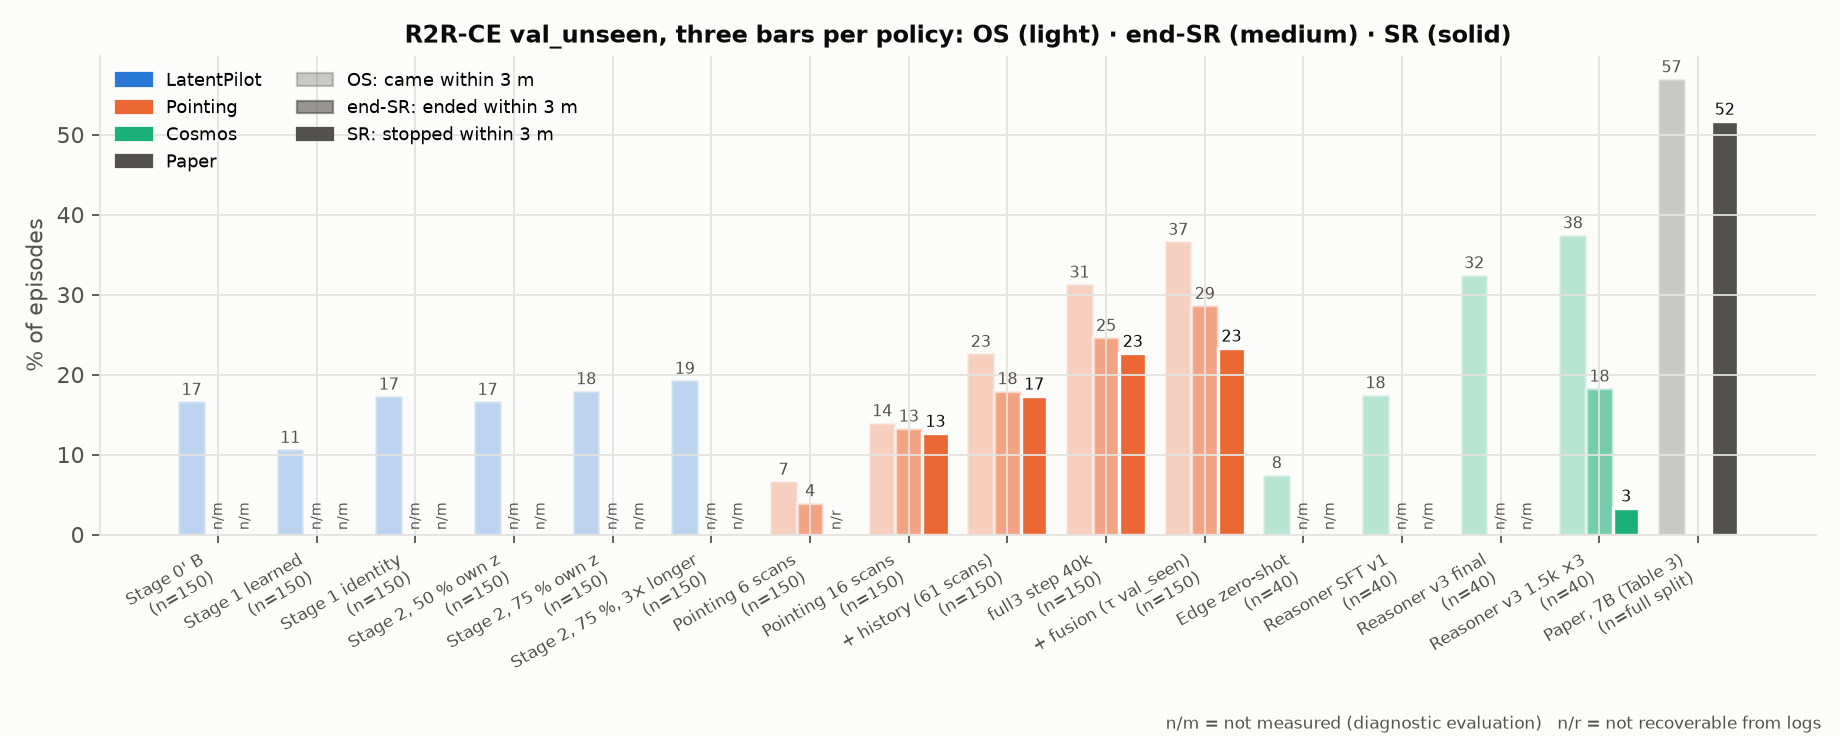
\includegraphics[width=\linewidth]{fig_navigation.png}
\caption{Oracle success (light) and strict self-stop success (solid) for every evaluated policy. Only the pointing
policy was evaluated strictly.}
\label{fig:nav}
\end{figure}

%---------------------------------------------------------------------------------------------------------------------
\subsection{LatentPilot: a better predictor, a worse navigator}
\label{sec:res-lp}

\paragraph{Stage 0 cannot be the paper's baseline.}
A memoryless Stage 0 policy reached 78\% training accuracy but never predicted STOP. In closed loop it spun in place:
10 of 12 episodes made zero progress, with 44\% LEFT and 43\% RIGHT actions against 62\% FORWARD in training. The paper's
supplement shows that its ``NaN'' baseline still carries the Pilot slot recurrently, so we built Stage 0$'$ to match it.

\paragraph{Slot placement: the zero-shot probe picked the wrong design.}
Untrained, Design A preserved 59.4\% instruction-following accuracy and Design B 29.4\%. After identical training
(\cref{fig:s0p}), A reached OS 0.0\% and B 16.7\% ($n{=}150$). Replacing B's slot content with a constant or the
current frame drops it to 0\%, while any learned content keeps 18--22\% ($n{=}60$). B's slot is therefore
load-bearing, and A's failure is architectural.

\begin{figure}[t]
\centering
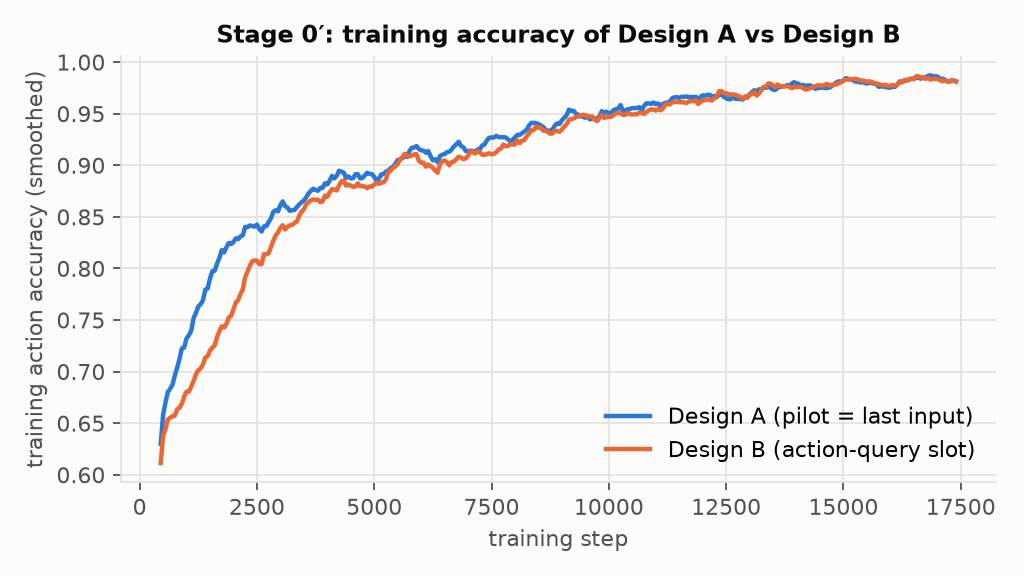
\includegraphics[width=0.6\linewidth]{fig_stage0prime.png}
\caption{Stage 0$'$ training accuracy for the two Pilot-slot designs. They are nearly identical in training but differ
completely in closed loop (OS 0.0\% vs.\ 16.7\%).}
\label{fig:s0p}
\end{figure}

\begin{figure}[t]
\centering
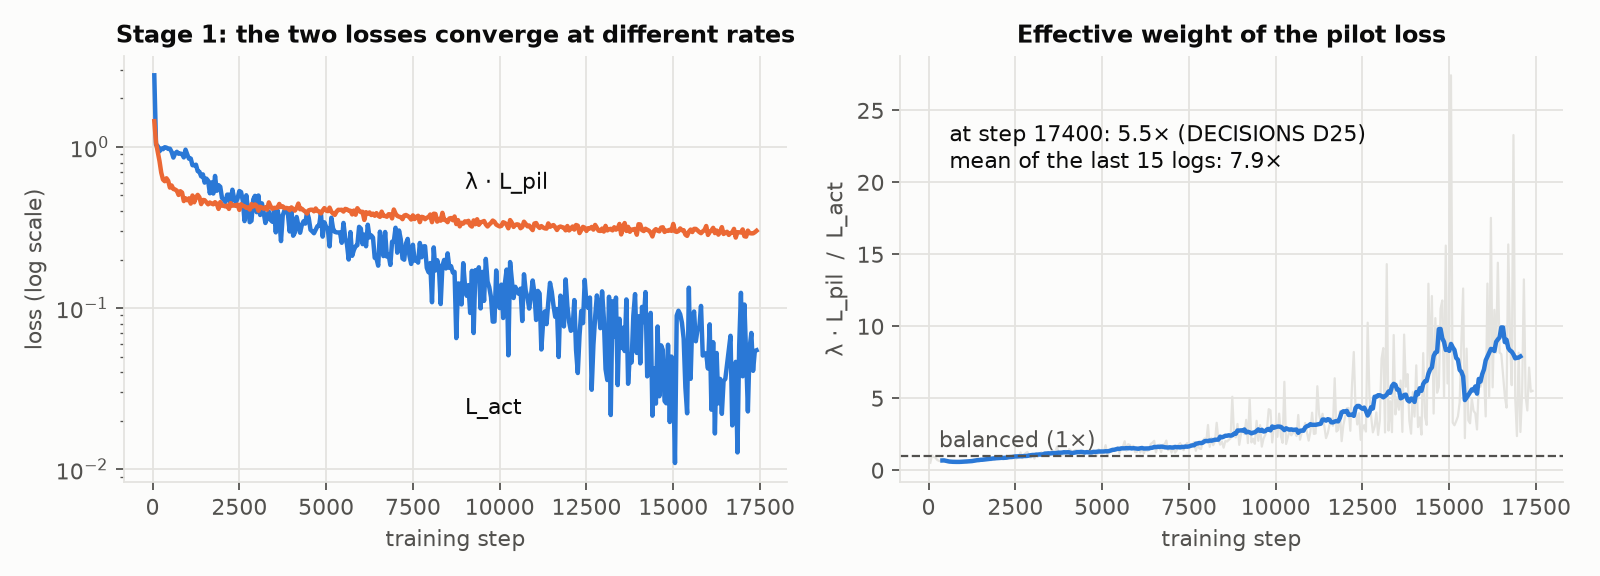
\includegraphics[width=\linewidth]{fig_loss_balance.png}
\caption{Stage 1 loss balance with $\lambda{=}0.1$. Left: the two loss terms. Right: their ratio
$\lambda\mathcal{L}_{pil}/\mathcal{L}_{act}$, which starts at about 0.5 and ends 5.5$\times$ larger.}
\label{fig:drift}
\end{figure}

\paragraph{The Stage 1 gate fails.}
\Cref{tab:lp} compares the learned $G_\psi$ against the identity control. The learned Pilot Token reaches a
2.25$\times$ lower $\mathcal{L}_{pil}$ (3.02 vs.\ 6.80; final training values), below the persistence baseline of 7.82.
It still reaches the goal less often. With $n{=}30$ the gap appeared as 10\% vs.\ 40\%; at $n{=}150$ it narrows to
10.7\% vs.\ 17.3\%, but it does not reverse.

\begin{table}[t]
\centering\small
\caption{LatentPilot Stage 0$'$ and Stage 1 (diagnostic; OS in \%). Stop = share of episodes ended by the model's
own STOP.}
\label{tab:lp}
\begin{tabular}{lcccccc}
\toprule
Model & $n$ & final $\mathcal{L}_{pil}$ & OS & nDTW & NE & stop \\
\midrule
Stage 0$'$, Design A (Pilot last) & 150 & \na & 0.0 & 0.244 & 8.79 & 39.3\% \\
Stage 0$'$, Design B (action query) & 150 & \na & 16.7 & 0.303 & 7.95 & 30.0\% \\
\midrule
Stage 1, learned $G_\psi$ & 30 & 3.02 & 10.0 & 0.306 & 8.58 & 0\% \\
Stage 1, identity $G_\psi$ & 30 & 6.80 & 40.0 & 0.404 & 7.40 & 0\% \\
Stage 1, learned $G_\psi$ & 150 & 3.02 & 10.7 & 0.277 & 8.50 & 4.7\% \\
Stage 1, identity $G_\psi$ & 150 & 6.80 & 17.3 & 0.268 & 8.17 & 0\% \\
Stage 1, adaptive $\lambda$ (step 10k) & 150 & \na & 6.7 & 0.275 & 8.36 & 18.0\% \\
\bottomrule
\end{tabular}
\end{table}

\paragraph{Diagnosis: loss-balance drift.}
With $\lambda=0.1$ the two terms of \cref{eq:lp} are balanced only at initialisation (\cref{fig:drift}).
$\mathcal{L}_{act}$ falls 51$\times$ over training while $\mathcal{L}_{pil}$ falls only 4.8$\times$. The ratio
$\lambda\mathcal{L}_{pil}/\mathcal{L}_{act}$ therefore grows from 0.52 to 1.03 at step 4k, 3.2 at step 10k and 5.5 at
the end, and most of the gradient ends up serving frame prediction.

An adaptive schedule that holds the ratio at 0.9, in the spirit of GradNorm~\citep{chen2018gradnorm}, removed the
drift ($\lambda$ fell from 0.17 to 0.04) but did not recover navigation (OS 6.7\% at step 10k). At 2B parameters and
1,665 episodes, predicting the future did not make a better navigator. This finding is specific to this scale and is
not a refutation of the 7B result.

%---------------------------------------------------------------------------------------------------------------------
\subsection{Pointing: the best true success rate}
\label{sec:res-pt}

\paragraph{Data is the binding constraint.}
Trained identically for 20k steps, the 6-scan policy reached strict SR 4.0\% although its training loss was lower
(0.076 vs.\ 0.396), while the 16-scan policy reached 13.3\% (\cref{tab:pt}). Moving to 61 scans with frame history
raised SR to 18.0\%, and a longer schedule to 24.7\%.

\begin{table}[t]
\centering\small
\caption{Pointing ablations, strict evaluation, $n{=}150$ (8 scans). $\tau$: STOP threshold. The history run used
stride 1 because of a launcher error.}
\label{tab:pt}
\begin{tabular}{lccccccc}
\toprule
Variant & scans & epochs & $\tau$ & SR & SPL & OS & NE \\
\midrule
final layer, no history & 6 & 2.30 & 0.05 & 4.0 & 3.7 & 6.7 & 8.37 \\
final layer, no history & 16 & 0.93 & 0.05 & 13.3 & 13.0 & 14.0 & 7.34 \\
+ history ($K{=}2$, stride 1) & 61 & 0.35 & 0.05 & 18.0 & 16.8 & 22.7 & 6.55 \\
+ history ($K{=}2$, stride 8), step 40k & 61 & 0.37 & 0.10 & 24.7 & 22.3 & 31.3 & 7.10 \\
+ layer fusion 23/26/28, step 120k & 61 & 1.10 & 0.20 & \textbf{31.3} & \textbf{25.4} & 42.7 & 7.22 \\
\midrule
\multicolumn{8}{l}{\emph{matched comparison at $\tau{=}0.20$:}} \\
final layer, step 60k (0.55 ep.) & 61 & 0.55 & 0.20 & 22.0 & 18.9 & 41.3 & 7.99 \\
layer fusion, step 80k (0.73 ep.) & 61 & 0.73 & 0.20 & 22.7 & 18.7 & 41.3 & 7.90 \\
\bottomrule
\end{tabular}
\end{table}

\paragraph{The policy uses the instruction, and STOP depends on it most.}
Teacher-forced on 900 held-out steps, action agreement is 0.764 with the true instruction, 0.686 with another
episode's, and 0.603 with none. The separation between STOP and non-STOP probabilities collapses from 5.1$\times$ to
1.0$\times$ once the instruction is swapped.

\paragraph{STOP lives mid-network.}
A linear probe on each of the 29 hidden states (2,000 training and 1,000 held-out frames) finds STOP at AUC 0.718 in
layer 15. At the final layer, which the head was reading, the AUC is 0.441, below chance (\cref{fig:probe}, left). A
head reading layers 23, 26 and 28 produced the best strict SR, 31.3\%.

A matched comparison at equal training shows little difference, however (22.7\% vs.\ 22.0\%, \cref{tab:pt}). Strict SR
over training is also non-monotonic (15.3, 30.0, 22.7, 18.7 and 31.3\% at 20k--120k; \cref{fig:thr}). The size of the
fusion effect is therefore not established.

\begin{figure}[t]
\centering
\begin{minipage}{0.56\linewidth}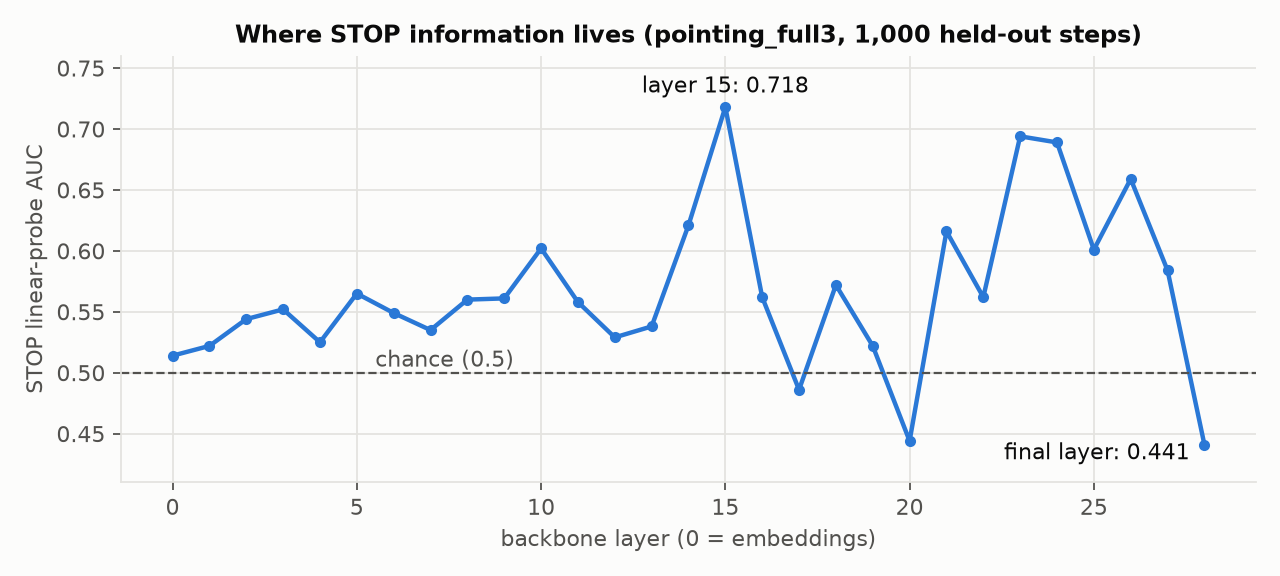
\includegraphics[width=\linewidth]{fig_layer_probe.png}\end{minipage}\hfill
\begin{minipage}{0.42\linewidth}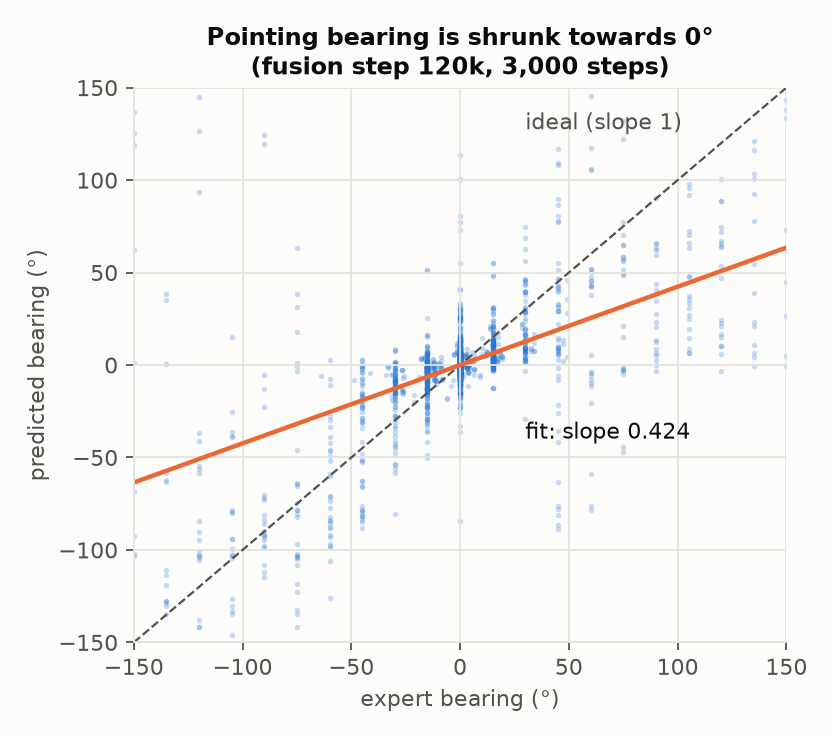
\includegraphics[width=\linewidth]{fig_bearing.png}\end{minipage}
\caption{Left: STOP linear-probe AUC per layer; the output layer is below chance. Right: the predicted bearing is
0.42$\times$ the expert's, so many turns fall under the 7.5\textdegree\ threshold.}
\label{fig:probe}
\end{figure}

\begin{figure}[t]
\centering
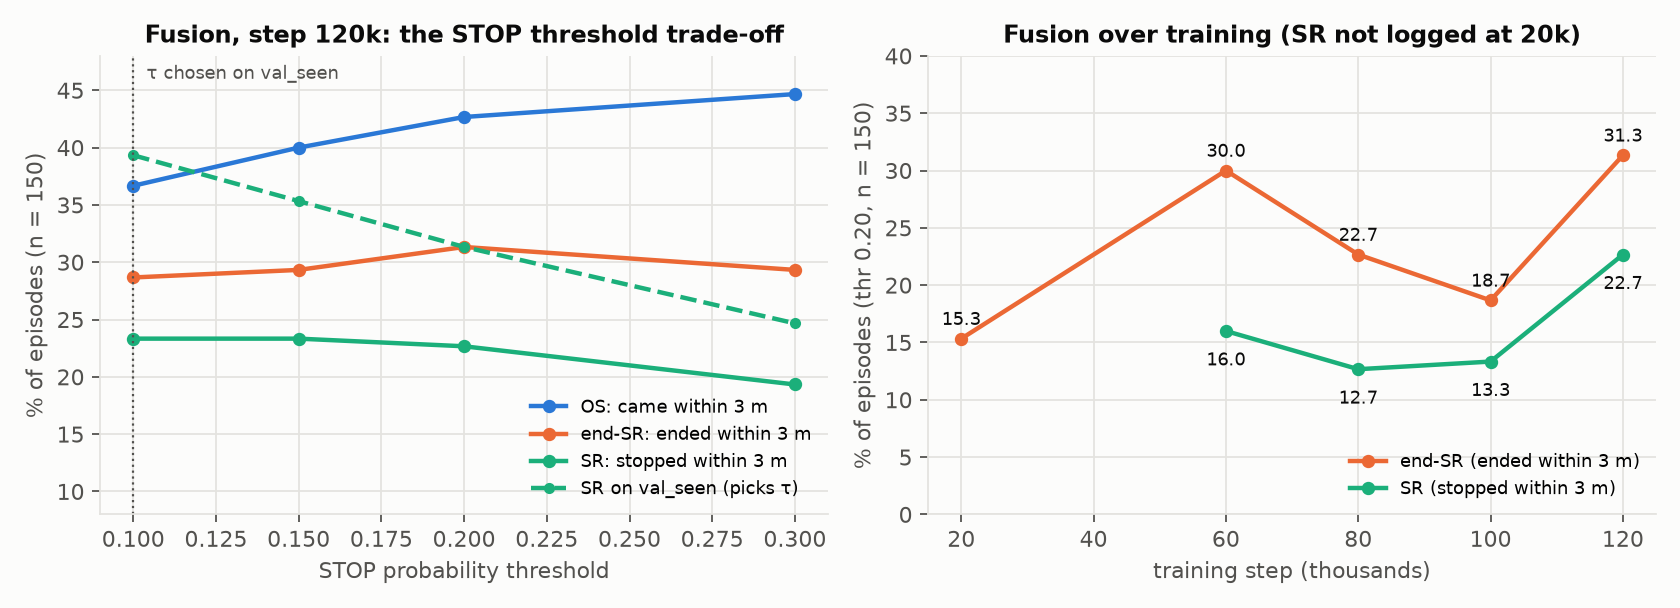
\includegraphics[width=0.9\linewidth]{fig_stop_threshold.png}
\caption{Pointing with layer fusion. Left: raising the STOP threshold $\tau$ trades premature stops for overshoots; OS
keeps rising while strict SR peaks at 0.20. Right: strict SR over training at $\tau{=}0.20$.}
\label{fig:thr}
\end{figure}

\paragraph{Why it still fails: under-turning and stopping.}
On 2,500 teacher-forced steps, agreement is 0.901 on FORWARD but only 0.55 on turns. Missed turns become FORWARD
(LEFT$\to$FWD 0.39, RIGHT$\to$FWD 0.43) and almost never go the wrong way (LEFT$\to$RIGHT 0.06). The cause is
regression shrinkage: the predicted bearing is 0.424$\times$ the true one (\cref{fig:probe}, right). Expert turns
average 41\textdegree\ but predictions average 27\textdegree.

Lowering the turn threshold does not help in closed loop (diagnostic OS of 35.3, 41.3, 42.0, 42.7 and 40.0\% at thresholds of 3, 4, 5, 7.5 and 10\textdegree), because a lower threshold produces zig-zagging. Recorded rollouts show three failure modes
(\cref{fig:qual}b,c): never approaching the goal, passing close to it without stopping, and stopping several metres
short.

%---------------------------------------------------------------------------------------------------------------------
\subsection{Cosmos3-Edge action model: motion prior without language}
\label{sec:res-edge}

\paragraph{Zero-shot inverse dynamics transfers.}
From our rendered walking video, the \texttt{av} (driving) domain recovers per-frame yaw with correlation 0.837 and
turn direction 96.4\% (384 frames, 11 scans). The \texttt{camera\_pose} domain reaches only 0.288. On video
re-rendered at a fixed 15\,fps, yaw correlation reaches 0.987, and the translation scale fits $s{=}7.47$
(forward correlation 0.92).

\paragraph{Instructions barely steer it.}
With short commands (``turn left''/``turn right'') the sign of the turn is correct 82/86/95/95\% of the time at
guidance 1/3/5/7.5 (\cref{fig:edge}). With full R2R instructions, turn direction agrees with the expert 59.4\% of the
time at guidance 1 (53.1\% with a swapped instruction), and 67.5\% vs.\ 49.5\% at guidance 7.5.

In closed loop ($n{=}40$) the policy reached OS 7.5\% and stopped in 75\% of episodes. A fixed prompt, ``The camera
moves forward.'', did at least as well (15.0\%, $n{=}20$). The motion prior is real, but the language has to come from
elsewhere.

\begin{figure}[t]
\centering
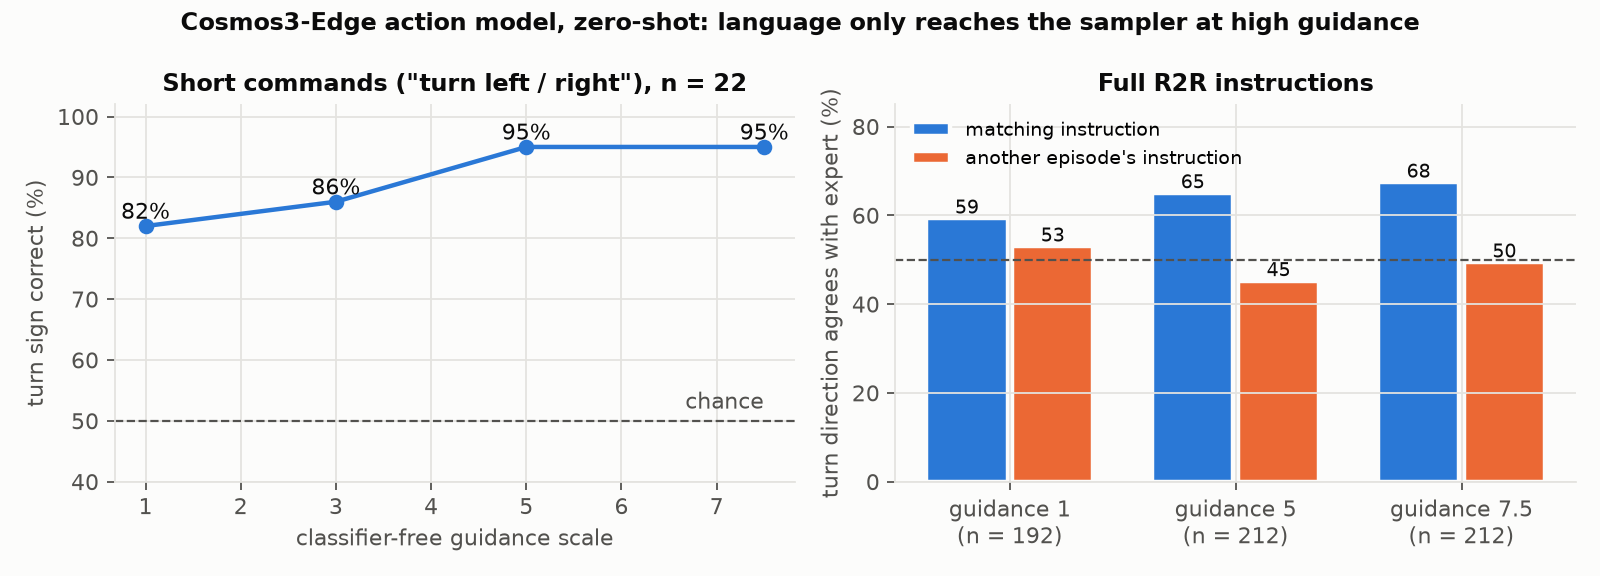
\includegraphics[width=0.95\linewidth]{fig_edge_guidance.png}
\caption{Cosmos3-Edge action model, zero-shot. Language influences the sampled motion only at high classifier-free
guidance, and full instructions steer it weakly.}
\label{fig:edge}
\end{figure}

%---------------------------------------------------------------------------------------------------------------------
\subsection{Cosmos3-Edge reasoner: reaching without stopping}
\label{sec:res-rs}

\paragraph{Zero-shot, it does not know it is the agent.}
Given a still frame, the reasoner produces plausible-looking waypoint lists (\cref{fig:rzs}). Asked for the next
action, however, it narrates the scene as a bystander. For the first frame in \cref{fig:rzs} it answered ``A person
enters the room through the archway, drawn by the reflection in the mirror or the painting's subject.'' With the
embodiment prompt, zero-shot next-action accuracy on 160 decision points is 32.5\% (33.1\% with thinking), below the
54.4\% majority baseline.

\begin{figure}[t]
\centering
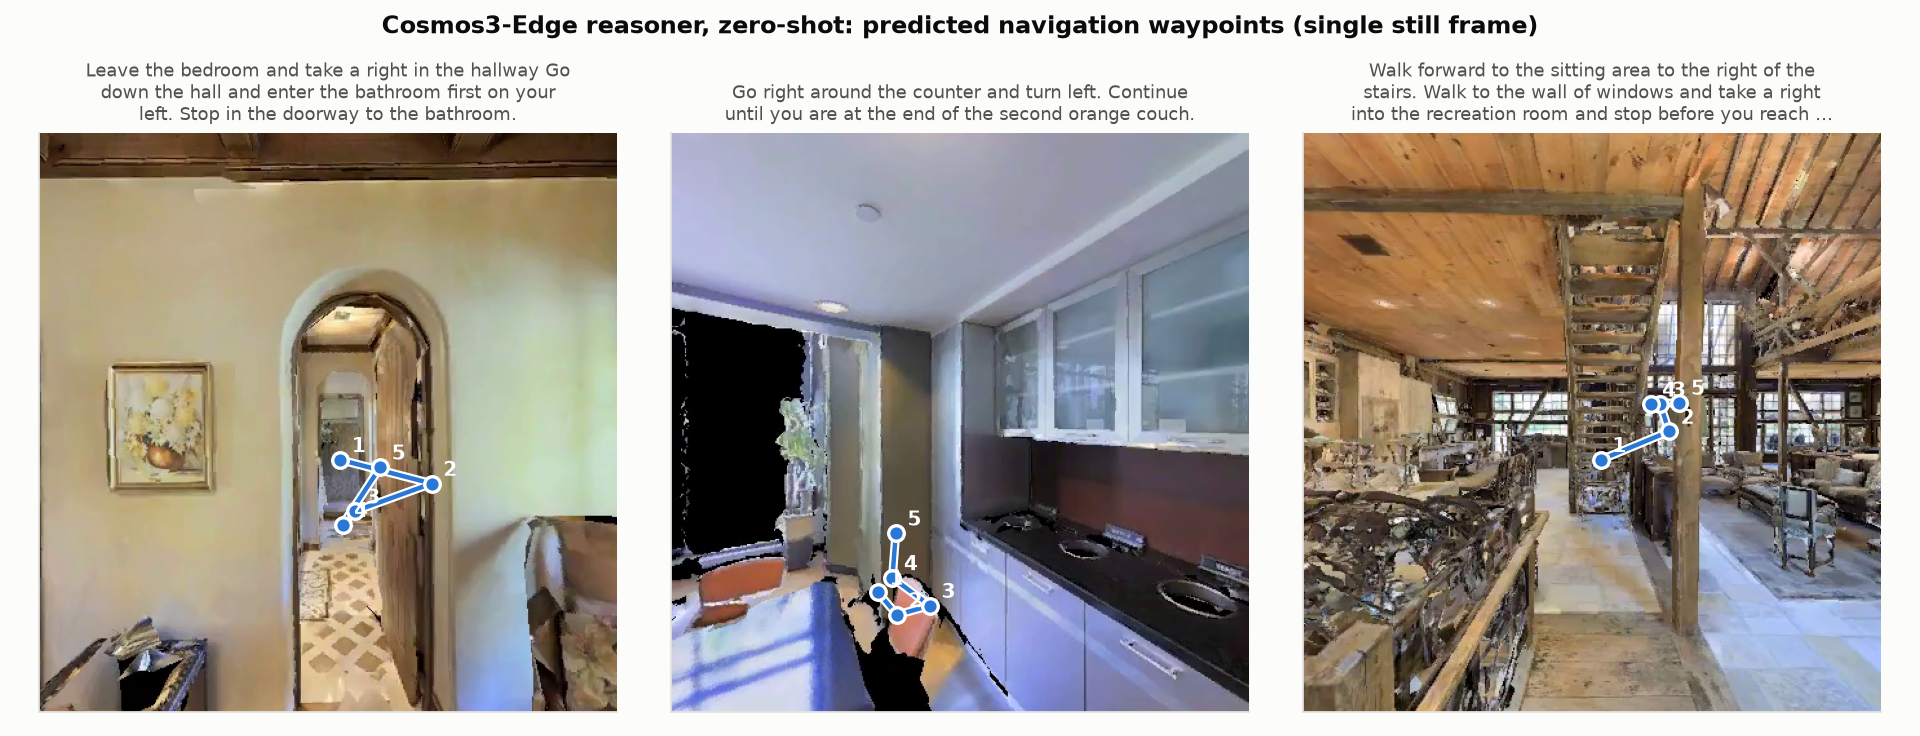
\includegraphics[width=\linewidth]{fig_reasoner_zeroshot.png}
\caption{Zero-shot reasoner: predicted navigation waypoints on single frames (coordinates normalised to 0--1000).}
\label{fig:rzs}
\end{figure}

\paragraph{Fine-tuning, and a probe that misleads.}
\Cref{tab:rs} compares probe accuracy with closed-loop success. SFT v1 has the best probe accuracy, 67.5\%, but in
closed loop it over-turns and over-stops: STOP ends 65\% of episodes, and its step-1,250 checkpoint reaches OS 0\%.
SFT v3 has lower probe accuracy (63.1\%, with STOP recall only 0.10) yet reaches OS 32.5\% at the final checkpoint and
\textbf{47.5\%} at step 1,500, the highest oracle success in this study. None of its five self-stops occurred within
3\,m of the goal, so its strict SR would be far lower. Because v3 changed three factors at once (sampling, context
length, projector), we cannot attribute its gain to any one of them.

\begin{table}[t]
\centering\small
\caption{Reasoner: offline next-action probe (160 decision points, majority baseline 54.4\%) vs.\ closed-loop OS
($n{=}40$, diagnostic).}
\label{tab:rs}
\begin{tabular}{lccccc}
\toprule
Model & context & probe acc. & closed-loop OS & nDTW & own STOP \\
\midrule
zero-shot (embodiment prompt) & 16 frames & 32.5 & \na & \na & \na \\
SFT v1, step 1,250 & 16 frames & 65.6 & 0.0 & 0.280 & 65\% \\
SFT v1, final & 16 frames & \textbf{67.5} & 17.5 & 0.365 & 65\% \\
SFT v3, final & 8\,s & 63.1 & 32.5 & 0.304 & 7.5\% \\
SFT v3, step 1,500 & 8\,s & \na & \textbf{47.5} & 0.389 & 12.5\% \\
\bottomrule
\end{tabular}
\end{table}

\begin{figure}[t]
\centering
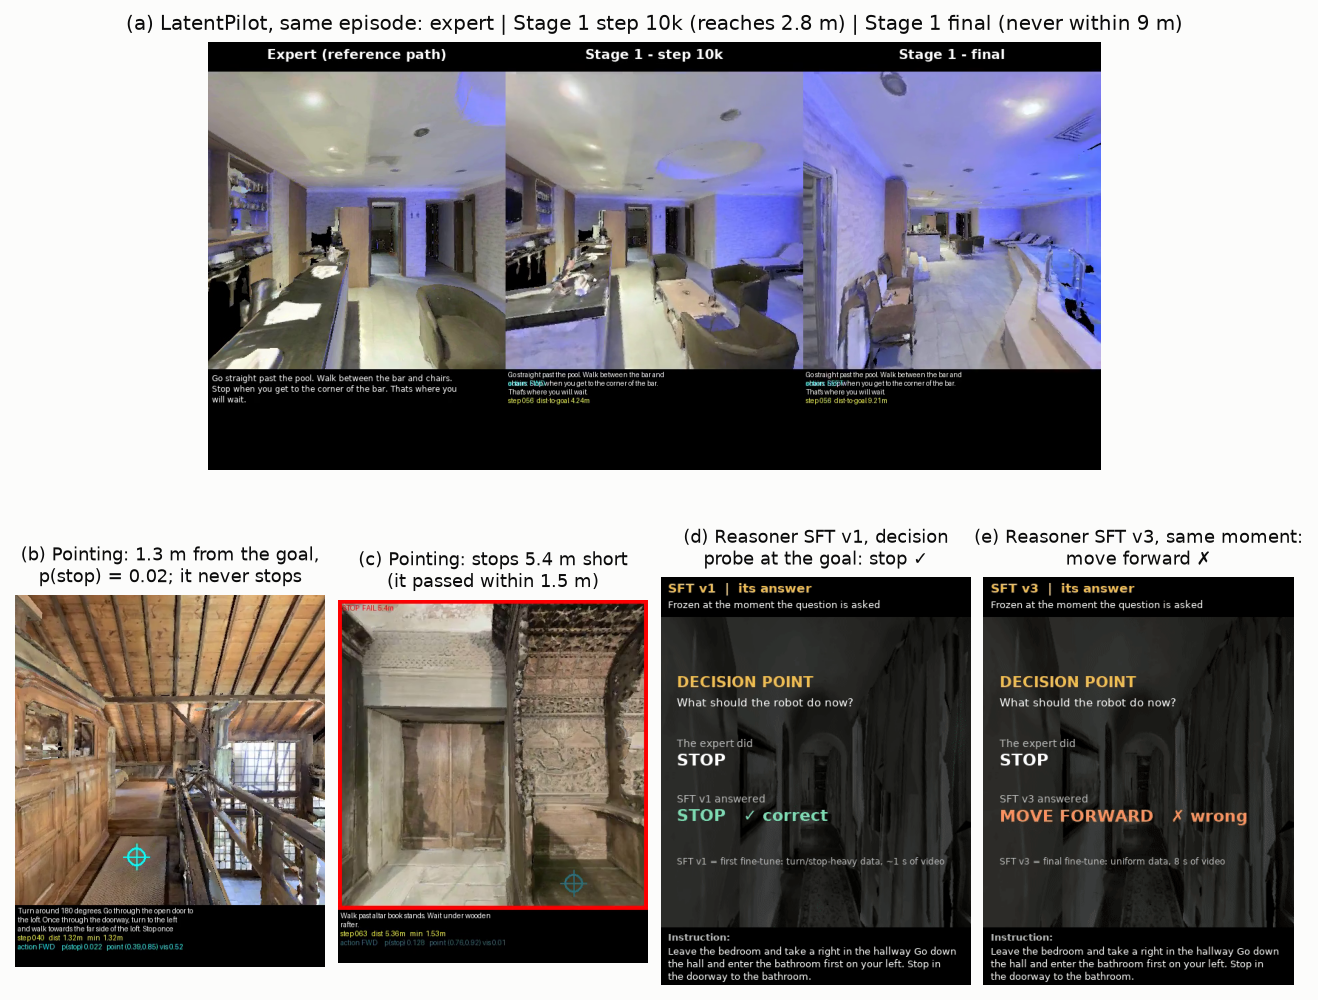
\includegraphics[width=\linewidth]{fig_qualitative.png}
\caption{Rollouts in unseen buildings. (a) LatentPilot: same episode for the expert, Stage 1 at 10k steps and the final
model. (b, c) Pointing failure modes. (d, e) Reasoner decision probes, not rollouts: each is the frame at which the model was asked for its next action
(the input is an expert's walk), with the expert's action and the answers of SFT v1 and v3. Videos are in the repository.}
\label{fig:qual}
\end{figure}

%=====================================================================================================================
\section{Discussion}
%=====================================================================================================================

\paragraph{Stopping is the bottleneck.}
Every approach reached the goal region more often than it stopped there. For the pointing policy the gap between OS
and SR is 11 points at its best threshold, and the reasoner never stopped inside 3\,m. The two sides of that failure
point to different fixes. The STOP signal exists in the backbone (layer-15 AUC 0.72), and it depends strongly on the
instruction. A dedicated STOP head is the one structural change that let a policy stop at all. We expect the next gains
to come from supervising STOP on progress through the instruction rather than on proximity alone.

\paragraph{Evaluate the claim, not a proxy.}
A diagnostic evaluation that ends on arrival made SR identical to OS for most of this project. Our first public
write-up reported one of these numbers as SR, and we have since corrected it. Offline probes also misled twice: a
zero-shot probe preferred the wrong Pilot-slot design, and the reasoner with the best next-action accuracy navigated
worst. Teacher-forced accuracy measures neither compounding error nor recovery, which is the exposure-bias
argument~\citep{bengio2015scheduled,ross2011dagger} in miniature.

\paragraph{Data and representation over architecture.}
The largest single improvements for the pointing policy came from more buildings (4.0$\to$13.3\%) and from correct
labels (0.69$\to$0.97 agreement). Frame history and layer fusion helped less clearly. The LatentPilot result is
consistent with this: an auxiliary objective cannot substitute for data at 6 buildings.

\paragraph{Pretrained video priors.}
Cosmos3-Edge's action stream carries a usable ego-motion prior but not instruction grounding. Its reasoner, once told
it is the agent and fine-tuned, is the strongest ``reacher''. Combining the two, with the reasoner deciding and the
diffusion model executing, was implemented but did not finish on our hardware (5 of 18 completed episodes reached the
goal region).

%=====================================================================================================================
\section{Limitations}
%=====================================================================================================================

Evaluations are small ($n{=}40$--150) and unpaired across approaches, and they cover 6--8 of the 11 unseen buildings.
STOP and turn thresholds were tuned on the evaluation split. Only the pointing policy was evaluated strictly. The
reasoner result is a single run with stochastic decoding. Several runs were stopped before finishing their schedules:
the long pointing runs completed 1.1--1.2 of 1.5--3 planned epochs. LatentPilot Stage 2 (scheduled sampling), a
16-scan Stage 1, and most arms of a prompt/policy ablation for the Cosmos models were never run. Our backbone (2B) and
data (6--61 buildings) differ from LatentPilot's (7B, full data), so our results describe this scale only.

%=====================================================================================================================
\section{Conclusion}
%=====================================================================================================================

On a single consumer GPU, supervising \emph{where to go} with a pointing head and a geometric controller gave the best
true success rate (31.3\%). A fine-tuned video reasoner reached the goal region most often (47.5\%) but did not stop
there. LatentPilot's dream-ahead objective and a zero-shot video diffusion policy did not produce competitive
navigators at this scale. In every case the limiting factor was the decision to stop, together with the gap between
what an offline metric measures and what the closed loop requires.

\paragraph{Reproducibility.}
Code, all training and evaluation logs, per-experiment notes, the scripts that regenerate every figure from the logs,
and rollout videos are at \url{https://github.com/ShubhJain007/vln-four-ways}. Matterport3D-derived media are for
non-commercial academic use under the Matterport3D terms of use.

\paragraph{Acknowledgements.}
Parts of the implementation, experiment orchestration and the drafting of this report were done with an AI coding
assistant (Claude, Anthropic). Every number reported here is taken from the logs in the repository.

\bibliographystyle{plainnat}
\bibliography{references}

\appendix
%=====================================================================================================================
\section{Reasoner prompt}
\label{app:prompt}
%=====================================================================================================================
The user turn is the concatenation of the following (verbatim from \texttt{src/nav/cosmos\_prompts.py}). The agent's
recent video is attached as a video input.

\begin{quote}\small\ttfamily\raggedright
You are a mobile robot navigating inside a building. The video depicts the observation from the robot's own
forward-facing camera at eye level, ending at the present moment.\\
This is the overall task that the agent is trying to complete: "\{instruction\}"\\
What should be the next action of the agent?\\
Choose the robot's next action. Answer with exactly one of: move forward, turn left, turn right, stop.
\end{quote}

%=====================================================================================================================
\section{Training configurations}
%=====================================================================================================================
\begin{table}[H]
\centering\small
\begin{tabular}{lL{2.6cm}L{3.2cm}L{2.5cm}L{3.3cm}}
\toprule
 & LatentPilot St.\ 1 & Pointing (fusion) & Edge action & Reasoner SFT v3 \\
\midrule
Base model & Cosmos-Reason2-2B & Cosmos-Reason2-2B & Cosmos3-Edge & Cosmos3-Edge (reasoner) \\
Trainable & LoRA r16 + $G_\psi$ & LoRA r16 + head (49k) & none (zero-shot) & LoRA r16 + projector (6.9M) \\
Data & 6 scans, 69.6k steps & 61 scans, 435k steps & \na & 45k decision points \\
Schedule & 17.4k steps $\times$ 8 & 124k of 163k steps $\times$ 4 & \na & 1 epoch, accum.\ 16 \\
LR & $10^{-4}$ cosine & $10^{-4}$ cosine & \na & $10^{-4}$ \\
Inference & argmax action & $\tau{=}0.20$, turn 7.5\textdegree & CFG 7.5, 20 steps, chunk 24 & top-$p$ 0.8, $T$ 0.7, 2-step bursts \\
\bottomrule
\end{tabular}
\end{table}

%=====================================================================================================================
\section{Full strict evaluation grid for the fusion policy}
%=====================================================================================================================
\begin{table}[H]
\centering\small
\caption{Every strict evaluation of the layer-fusion pointing policy ($n{=}150$, turn threshold 7.5\textdegree).}
\begin{tabular}{lcccccc}
\toprule
Step & $\tau$ & SR & SPL & OS & nDTW & NE \\
\midrule
20k & 0.05 & 4.0 & 4.0 & 6.0 & 0.328 & 7.90 \\
20k & 0.10 & 8.7 & 7.3 & 10.0 & 0.315 & 7.92 \\
20k & 0.20 & 15.3 & 11.7 & 19.3 & 0.286 & 7.77 \\
\midrule
60k & 0.20 & 30.0 & 24.3 & 48.0 & 0.278 & 7.13 \\
60k & 0.35 & 24.7 & 17.3 & 50.0 & 0.196 & 7.50 \\
60k & 0.50 & 23.3 & 15.2 & 50.0 & 0.178 & 7.60 \\
\midrule
80k & 0.15 & 20.7 & 17.0 & 37.3 & 0.269 & 7.89 \\
80k & 0.20 & 22.7 & 18.7 & 41.3 & 0.248 & 7.90 \\
80k & 0.30 & 19.3 & 14.1 & 45.3 & 0.178 & 8.32 \\
\midrule
100k & 0.15 & 20.0 & 18.1 & 37.3 & 0.295 & 8.27 \\
100k & 0.20 & 18.7 & 16.1 & 40.0 & 0.258 & 8.45 \\
100k & 0.30 & 16.7 & 13.4 & 44.0 & 0.189 & 8.85 \\
\midrule
120k & 0.10 & 28.7 & 24.3 & 36.7 & 0.363 & 7.03 \\
120k & 0.15 & 29.3 & 24.4 & 40.0 & 0.351 & 7.05 \\
120k & 0.20 & \textbf{31.3} & \textbf{25.4} & 42.7 & 0.323 & 7.22 \\
120k & 0.30 & 29.3 & 23.6 & 44.7 & 0.287 & 7.59 \\
\bottomrule
\end{tabular}
\end{table}

\end{document}
